%%%%%%%%%%%%%%%%%%%%%%%%%%%%%%%%%
%
%       EXERCÍCIO
%
%%%%%%%%%%%%%%%%%%%%%%%%%%%%%%%%%

\ifdefstring{\atividade}{prova}{%
    \ifdefstring{\modo}{objetivo}{%
        \renewcommand{\valorquestao}{\ValorQObj\ ponto}
    }{%
        \renewcommand{\valorquestao}{\ValorQDisc\ pontos}
    }%
}%

\begin{exercicioBanco}[\valorquestao]
Os gráficos abaixo representam as funções arrecadação \(A(x)\) e custo operacional \(C(x)\) de um evento, em que \(x\) é o número de ingressos vendidos. Determine o lucro obtido ao vender \(800\) ingressos, onde o lucro é a diferença entre a arrecadação e o custo operacional.

\begin{center}
    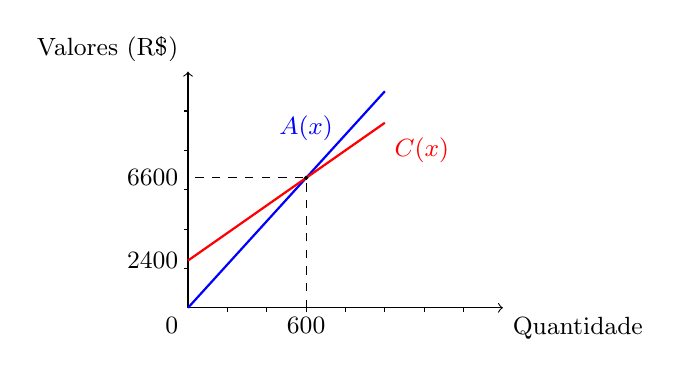
\begin{tikzpicture}[scale=0.5]

        % Eixos
        \draw[->] (0,0) -- (8,0) node[below right] {\small Quantidade};
        \draw[->] (0,0) -- (0,6) node[above left] {\small Valores (R\$)};

        % A(x)
        \draw[domain=0:5, smooth, variable=\x, blue, thick] 
            plot ({\x}, {1.1*\x});
        \node[blue, above] at (3,4) {\small \(A(x)\)};

        % C(x)
        \draw[domain=0:5, smooth, variable=\x, red, thick] 
            plot ({\x}, {0.7*\x + 1.2});
        \node[red, right] at (5,4) {\small \(C(x)\)};

        % Ponto de interseção (aproximado)
        \filldraw (3,3.3) circle (1.2pt);
        
        \draw[dashed] (3,0) -- (3,3.3) -- (0,3.3);
        \node[below] at (3,0) {\small \(600\)};
        \node[left] at (0,3.3) {\small \(6600\)};
        \node[below left] at (0,0) {\small \(0\)};
        \node[left] at (0,1.2) {\small \(2400\)};

        % Marcas nos eixos
        \foreach \x in {1,2,3,4,5,6,7}
            \draw (\x,0) -- (\x,-0.1);

        \foreach \y in {1,2,3,4,5}
            \draw (0,\y) -- (-0.1,\y);

    \end{tikzpicture}
\end{center}

% Define as alternativas
\newcommand{\alternativas}{%
    \begin{center}
        \begin{tabularx}{\textwidth}{XXXXX}
            (a) R\$ \(100{,}00\). &
            (b) R\$ \(400{,}00\). &
            (c) R\$ \(500{,}00\). &
            (d) R\$ \(800{,}00\). &
            (e) R\$ \(1000{,}00\).
        \end{tabularx}
    \end{center}
}

% Resposta correta
\newcommand{\resposta}{D}

% Lógica condicional para exibição
\ifdefstring{\atividade}{lista}{%
    \alternativas
    \vspace{0.5em}
    
    \noindent\textbf{Resposta:} letra \textbf{\resposta}.
}{%
    \ifdefstring{\modo}{objetivo}{%
        \alternativas
    }{%
        % modo = discursiva → não mostra alternativas
    }
}
\end{exercicioBanco}

